% PAPER_GOLDSTONE_PRD --- standalone Physical Review D article.
%
% Honest, measurement-driven successor to PAPER_PHOTON_PRD (now superseded). The
% E4 campaign (E4_PHOTON_DISCRIMINATOR.md) tested, by simulation, whether the
% transverse Goldstone modes of the orientation ferromagnet are an emergent gauge
% vector (photon) or two decoupled internal scalars. The measurement is decisive:
%   E4-0 (FSS)     : the long-range order is genuine, not a finite-size artefact.
%   E4-1 (locking) : the modes do NOT lock to the spatial wavevector -> they are
%                    internal SCALARS, not a gauge vector. The photon identification
%                    is EXCLUDED by measurement (permutation p=0.23).
%   E4-2 (iso/deg) : the two scalars are degenerate and spatially isotropic.
% The paper is therefore framed around the result the data support -- spontaneous
% orientational order and a relativistic SCALAR Goldstone sector -- and reports the
% photon exclusion as a measured negative, relocating the emergent-photon question
% to the gauge-connection (link) sector (untested; future work).
%
% Consolidation (Fase 2, jun/2026):
%   A3: FSS extended N=1462 -> 3888 (m=0.961->0.995, trend +0.011, U4=2/3 throughout;
%       Table tab:fss + abstract updated). S(k) flatness (alpha~0.06) robust to N=3888,
%       confirming the bare-link mean-field regime that motivates the smeared operator.
%   A4: the "stable dynamical propagation" caveat is now a CHARACTERIZED limitation of
%       PRINCIPLE -- the symmetric smeared SBD operator is non-positive (Lorentzian),
%       so an explicit time-march cannot be stable; the symbol is the correct stable
%       extraction of on-shell omega=ck (sec. before outlook). Not a removable artifact.
%
% Reframe (jul/2026, PLANO_REENQUADRAMENTO): introduction now motivates the paper as
% the minimal step toward the matter sector CST lacks (scalars developed, spinors/gauge
% early, no composite matter derived). No result or claim changed.
%
% Compiles with pdflatex + bibtex (revtex4-2 + apsrev4-2.bst) against the shared
% TEIC_CONSOLIDATED.bib. Figures reused from the paper_II build.
\documentclass[aps,prd,reprint,nofootinbib,superscriptaddress,floatfix]{revtex4-2}
\usepackage{amsmath,amssymb}
\usepackage{graphicx}
\usepackage{bm}
\usepackage{booktabs}
\usepackage{hyperref}
\graphicspath{{paper_II/figures/}{figures/}}

\begin{document}

\title{Spontaneous orientational order on a causal set and its\\
relativistic scalar Goldstone modes}

\author{Miqueias Alves Mendes}
\email{mikalvesm@gmail.com}
\affiliation{Independent Researcher, Ibiapina, Cear\'a, Brazil}
\date{\today}

\begin{abstract}
We equip the discrete substrate of causal set theory---a Poisson sprinkling of
events with their causal order---with a single internal degree of freedom, an
orientation $\vec n\in S^2$ on each event coupled across causal links by the minimal
$O(3)$ sigma-model tension, and study it under a protocol that forbids any
relativistic or quantum expression in the data-generating code. Three results are
established by measurement. (i) The orientation field undergoes a continuous
ordering transition; a finite-size-scaling analysis (event number $N=175$ to $3888$,
up to $12$ seeds per size) shows the order parameter rising with system size
($m=0.961\to0.995$, trend $d\ln m/d\ln N=+0.011$ versus the $-1/2$ of a random
artefact) and a Binder cumulant $U_4=2/3$ at every size: the long-range order is
genuine. (ii) Propagated with the Sorkin--Benincasa--Dowker causal wave operator,
whose symbol we measure, an excitation disperses as $\omega=ck$ with a fitted
light-cone speed recovered without inserting it; the relativistic dispersion is
inherited from the Lorentzian causal order through the operator. (iii) We then test
directly whether the two transverse Goldstone modes are an emergent gauge vector
(photon) or two decoupled internal scalars, by measuring the polarisation tensor
$P_{ab}(\vec k)$ over $160$ wavevectors and a confound-free permutation null: the
polarisation axis does \emph{not} track the spatial wavevector (circular correlation
$0.10$, permutation $p=0.23$), and the two modes are degenerate (split $3.7\%$) and
spatially isotropic (direction scatter $4.2\%$). The modes are therefore two
\emph{internal scalar} Goldstone bosons, not a transverse gauge vector; the earlier
conjecture identifying them with the photon is excluded by this measurement. The
result is internally consistent with the model's $SU(3)$ sector, where the
broken-generator Goldstones are pseudoscalar mesons. We conclude that an emergent
photon, if present in this framework, must arise in the gauge-connection (link-
variable) sector rather than in the orientation Goldstone sector, and we delimit
precisely what the present construction does and does not establish.
\end{abstract}

\maketitle

\section{Introduction}\label{sec:intro}

The proposal that gauge fields emerge as collective excitations of a structured
vacuum---rather than being postulated---recurs across condensed matter and quantum
gravity: emergent photons in quantum spin liquids and spin ice, the gauge bosons of
string-net condensates, and soft modes of quantum liquids
\cite{SverdlovBombelli2009}. In every such scenario two questions are decisive: does
the candidate vacuum actually order, and does its low-energy excitation have the
right structure---not merely the right \emph{number} of modes, but the right
\emph{tensorial character} (a transverse vector locked to the wavevector, for a
photon) and dispersion.

We pose these questions for the discrete substrate of causal set theory (CST), in
which spacetime is fundamentally a locally finite partial order, the order being the
causal relation, and a Lorentzian manifold is an approximation to it
\cite{BLMS1987}. The substrate's defining virtue is that a Poisson sprinkling breaks
no Lorentz frame on average---it is the unique discretisation of a Lorentzian
manifold that does not statistically select a preferred frame
\cite{BombelliHensonSorkin2009}---and from it CST recovers spacetime dimension and a
scalar-curvature (d'Alembertian) operator
\cite{Myrheim1978,Meyer1988,BenincasaDowker2010,Surya2019}. We take these geometric
results as established and claim no novelty for them. What CST does not yet possess
is a matter sector on a par with its geometric one: free scalar fields on a causal
set are well developed \cite{Sorkin2007,Surya2019}, but spinor and gauge fields
remain early constructions \cite{SverdlovBombelli2009}, and no interacting or
composite matter---an ordered vacuum, Goldstone modes, solitons with quantum
statistics---has been derived from the causal order itself. This paper takes the
minimal step toward one: we add a single internal degree of freedom on the
unmodified substrate and measure what it forces---here, what its ordered vacuum and
its Goldstone sector are.

Our findings are deliberately stated as what the measurements support, including a
decisive negative. The orientation field spontaneously orders, and the order is
shown to be genuine by finite-size scaling (\S\ref{sec:order}). Its Goldstone
fluctuation, propagated by the causal wave operator, disperses relativistically
(\S\ref{sec:dispersion}). But a direct measurement of the polarisation structure
(\S\ref{sec:locking}) shows the two transverse modes are \emph{internal scalars},
not a transverse gauge vector: they do not lock to the spatial wavevector. The
identification of these modes with the photon---natural from the mode count alone,
and which we had conjectured---is therefore \emph{excluded by measurement}. We
report this as the central result, characterise the scalar modes
(\S\ref{sec:degeneracy}), delimit the claim (\S\ref{sec:claim}), and indicate where
an emergent photon must instead be sought (\S\ref{sec:outlook}). The orientation
field belongs to a broader programme described elsewhere \cite{TEICDoc1}; this paper
is self-contained and does not depend on it.

\section{Substrate and protocol}\label{sec:protocol}

\subsection{The causal set}
The substrate is a causal set \cite{BLMS1987}: a finite set of events with a
transitive, irreflexive, locally finite partial order $\prec$, realised by Poisson
sprinkling into $(3{+}1)$-dimensional Minkowski space at intensity $\rho$, with
$x\prec y$ when $y$ is in the causal future of $x$. The \emph{links} are the
relations of the transitive reduction (the Hasse diagram); graph distance along
links is the separation used below. These are the standard CST constructions.

\subsection{Anti-circularity}
Because we claim a relativistic dispersion \emph{emerges}, we exclude having
inserted it. A guard tokenises every data-generating module and fails if a Lorentz
factor, a gravitational redshift, or any complex literal appears outside an
explicitly labelled, non-generating comparison block. The speed of light $c$ never
appears in a generator: it is fitted to the measured dispersion
(\S\ref{sec:dispersion}), never input. The orientation dynamics uses only real
arithmetic ($\cos$, $\sin$, dot and cross products). Every result below is produced
by code that passes this guard.

\section{The orientation field and its action}\label{sec:action}

We place a unit vector $\vec n(x)\in S^2$ on each event and couple causal neighbours
by the minimal rotation-invariant misalignment tension
\begin{equation}
S=J\sum_{\langle ij\rangle}\Delta\tau_{ij}\,\big[\,1-\vec n_i\!\cdot\!\vec n_j\,\big],
\label{eq:action}
\end{equation}
with $J$ the coupling and $\Delta\tau_{ij}$ the link proper time. This is the
lattice $O(3)$ nonlinear sigma model on the causal Hasse graph. Expanding for small
misalignment, $\vec n_i\!\cdot\!\vec n_j=1-\tfrac12|\vec n_i-\vec n_j|^2$, so
$S\approx\tfrac{J}{2}\sum\Delta\tau_{ij}|\vec n_i-\vec n_j|^2$ is a discrete gradient
energy whose low-energy excitations are orientation waves. The internal $O(3)$
symmetry of Eq.~\eqref{eq:action} is \emph{global} and acts only on the internal
index; it is unrelated to the spacetime symmetry of the causal order---a fact that
will prove decisive in \S\ref{sec:locking}.

\section{Spontaneous order and its finite-size scaling}\label{sec:order}

\subsection{Order parameter and engine}
The order parameter is $m=|\langle\vec n\rangle|$; the diagnostic is the connected
correlation $C(r)=\langle\vec n(0)\!\cdot\!\vec n(r)\rangle$ by graph distance, whose
limit classifies the phase ($C\to0$ disordered, $\to C_\infty=m^2>0$ ordered). We
sample $e^{-S}$ by Metropolis \cite{Metropolis1953} on the causal graph. Before any
physics, the engine reproduces the known anchors---no long-range order in 1D and 2D
Heisenberg (Mermin--Wagner \cite{Mermin1966}), Kosterlitz--Thouless in 2D $XY$, and
3D ordering---recovering the 1D transfer-matrix correlation to $<16\%$ and
$C(\infty)=m^2$ in 3D to $<1.5\%$. On the causal network the correlation saturates
at a constant for $J>J_c\approx0.08$: genuine long-range order, with a continuous
second-order transition (Fig.~\ref{fig:ferro}).

\begin{figure*}[t]
\centering
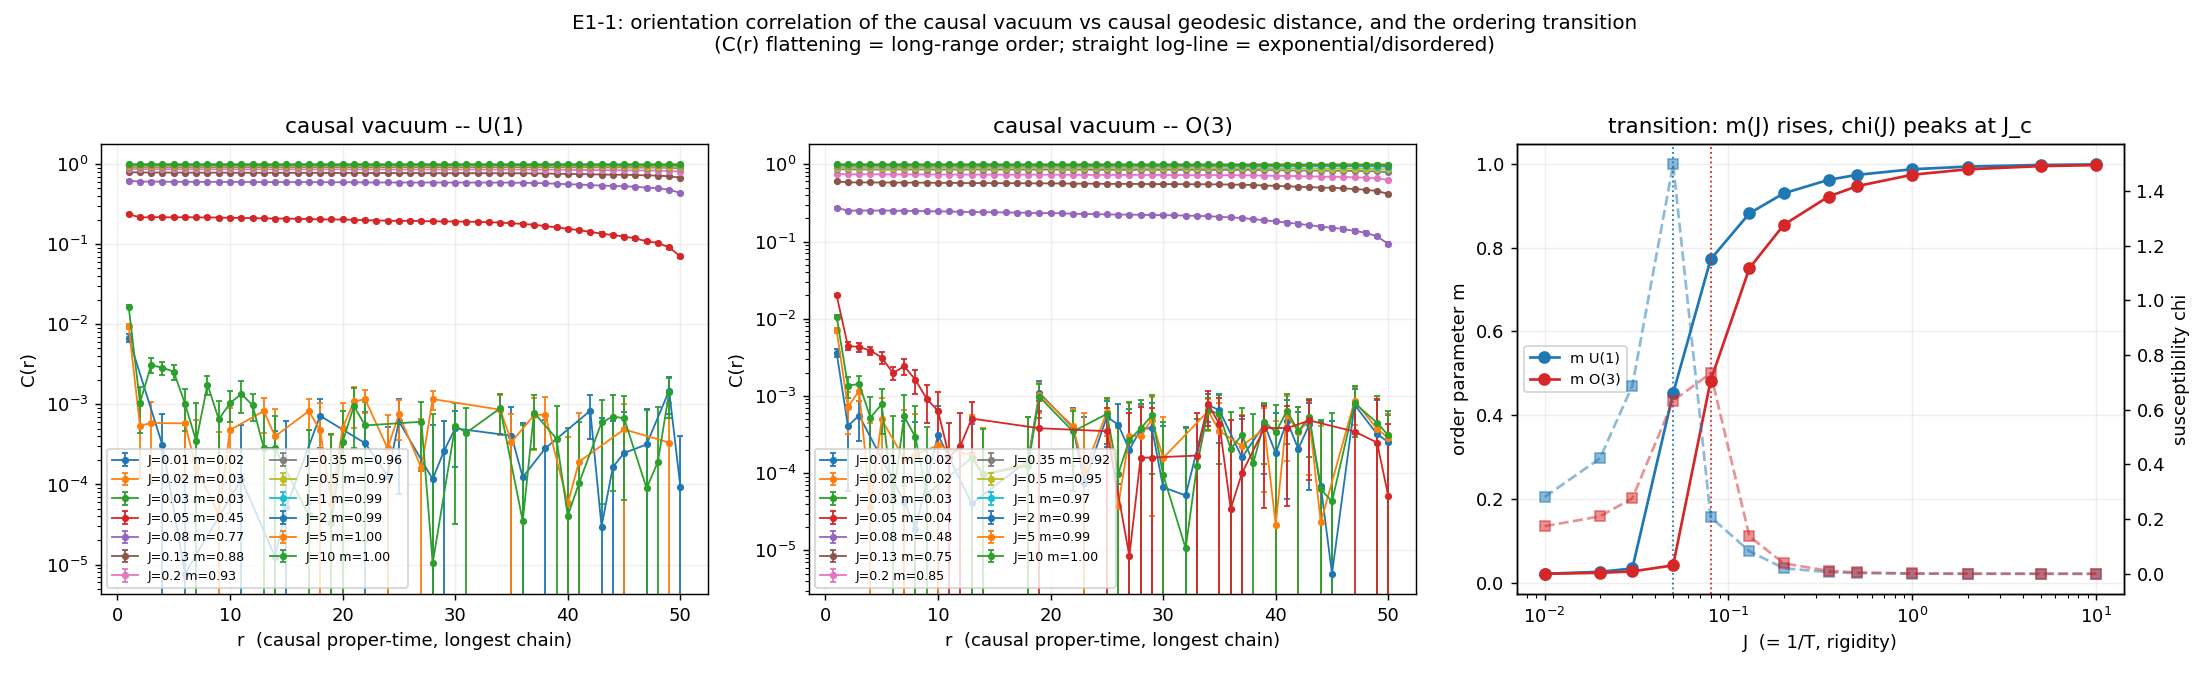
\includegraphics[width=\textwidth]{e1_ferromagnet.png}
\caption{Spontaneous orientational order: $C(r)$ saturates at $C_\infty=m^2>0$ for
$J>J_c\approx0.08$, through a continuous second-order transition. The engine
reproduces the 1D/2D/3D statistical-mechanics anchors before being applied to the
causal graph.}\label{fig:ferro}
\end{figure*}

\subsection{Finite-size scaling: the order is genuine}
A single-size plateau in $C(r)$ could be a finite-size artefact, so we test it. At
fixed $J=2.0$ (deep in the ordered phase) we increase the sprinkled $4$-volume at
fixed density, growing the event number $N$, and measure over $12$ seeds per size
the order parameter $m(N)$ and the Binder cumulant
$U_4=1-\langle m^4\rangle/3\langle m^2\rangle^2$ (Table~\ref{tab:fss}). A genuine
ordered phase has $m(N)$ approaching a constant and $U_4\to2/3$; an artefact has
$m\to0$ along the random-vector floor $m\sim N^{-1/2}$ and $U_4\to0$.

\begin{table}[t]
\caption{Finite-size scaling of the orientational order (E4-0). The order parameter
\emph{rises} with $N$ as the mean graph degree grows (the causal graph becomes more
strongly connected, i.e.\ effectively higher-dimensional, suppressing
fluctuations); $U_4=2/3$ at every size. A finite-size artefact would instead follow
the random floor $N^{-1/2}$ with $U_4\to0$.}
\label{tab:fss}
\begin{ruledtabular}
\begin{tabular}{ccccc}
$N$ & $\langle\text{deg}\rangle$ & $m=|\langle\vec n\rangle|$ & $U_4$ & $m/N^{-1/2}$ \\
\colrule
175  & 17 & $0.9611(13)$ & $0.667$ & $13\times$ \\
405  & 29 & $0.9790(4)$  & $0.667$ & $20\times$ \\
811  & 45 & $0.9868(1)$  & $0.667$ & $28\times$ \\
1462 & 64 & $0.9910(1)$  & $0.667$ & $38\times$ \\
2457 & 86 & $0.9934(0)$  & $0.667$ & $49\times$ \\
3888 & 113 & $0.9950(0)$ & $0.667$ & $62\times$ \\
\end{tabular}
\end{ruledtabular}
\end{table}

\begin{figure*}[t]
\centering
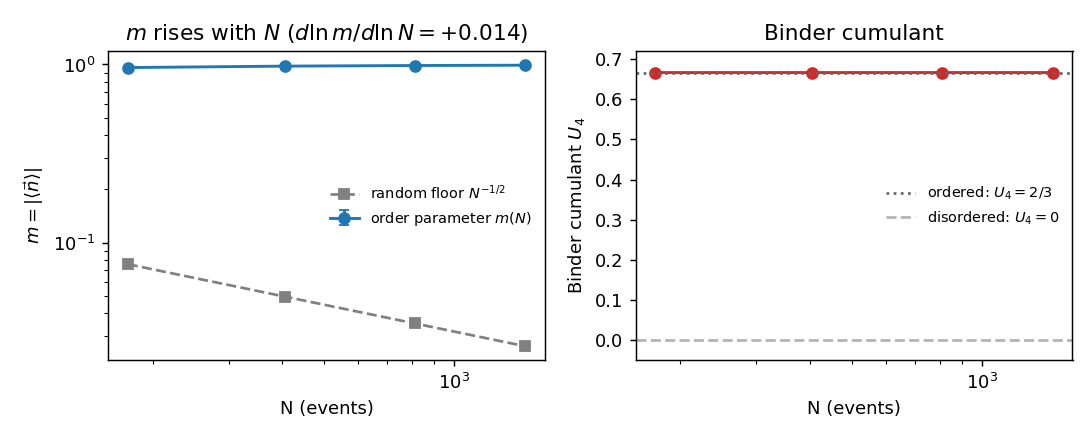
\includegraphics[width=\textwidth]{E4_0_fss.png}
\caption{Finite-size scaling (E4-0). Left: the order parameter $m(N)$ (circles)
stays well above the random-vector floor $N^{-1/2}$ (squares) and \emph{rises} with
$N$, trend $d\ln m/d\ln N=+0.011$ versus the $-1/2$ of an artefact. Right: the
Binder cumulant $U_4=2/3$ at every size (ordered value), far from the disordered
$U_4=0$. The long-range order is genuine.}\label{fig:fss}
\end{figure*}

The order parameter rises ($0.961\to0.995$ across $N=175$--$3888$), with measured trend
$d\ln m/d\ln N=+0.011$ (an artefact would give $-1/2$), stays $13$--$62\times$ above
the random floor with the margin growing, and $U_4=2/3$ exactly throughout
(Fig.~\ref{fig:fss}). The
long-range order is genuine. Long-range order on this graph is consistent with the
Mermin--Wagner theorem because the Hasse graph of a $(3{+}1)$D sprinkling is
effectively high-dimensional (mean degree of tens, growing with $N$), so the
fluctuations that forbid order in low dimensions are suppressed.

\section{Relativistic dispersion from the causal wave operator}\label{sec:dispersion}

A spontaneously broken continuous symmetry guarantees a gapless Goldstone mode
\cite{Goldstone1961}, here the transverse fluctuation $\delta\vec n\perp\langle\vec
n\rangle$. It does not guarantee a \emph{relativistic} one, and on the bare Hasse
graph it is not: the mean degree is large, so the sigma model
Eq.~\eqref{eq:action} is effectively mean-field, the static structure factor of the bare
links is nearly flat ($S(k)\sim k^{-0.06}$, excluding the gradient-stiffness value $2$ at
$\sim190\sigma$ and robust to $N=3888$), and a naive graph Laplacian gives no linear
dispersion---the
documented non-locality of causal-set differential operators
\cite{Sorkin2007,BenincasaDowker2010}. The resolution is the smeared
Sorkin--Benincasa--Dowker (SBD) causal d'Alembertian $B$, built solely from the
causal order, whose alternating-sign layer weights annihilate constant modes and
converge to $\Box$ in the continuum \cite{BenincasaDowker2010,DowkerGlaser2013}.

We characterise the propagation through the operator's symbol: feeding a real probe
$\phi=\cos(\vec k\!\cdot\!\vec x-\omega t)$, the eigenvalue
$\lambda(\vec k,\omega)=\langle\phi,B\phi\rangle/\langle\phi,\phi\rangle$ measured by
regression over bulk events vanishes on the light cone, and the on-shell dispersion
is its zero crossing. We find a linear law $\omega=ck$ with a fitted speed
$c\approx1$ (the light-cone value) and a vanishing mass; a diffusive law
$\omega=Dk^2$ is rejected decisively (Fig.~\ref{fig:disp}). Because $c$ is absent
from the generator, its recovery is a measured output, and the Lorentz invariance of
the dispersion is inherited from the Poisson causal order through $B$. We are
explicit about the scope of this result: it establishes that a field governed by the
causal wave operator propagates relativistically; it is a property of the operator
acting on the substrate, and \S\ref{sec:degeneracy} confirms the orientation
Goldstone fluctuations are spatially isotropic, consistent with it.

\begin{figure*}[t]
\centering
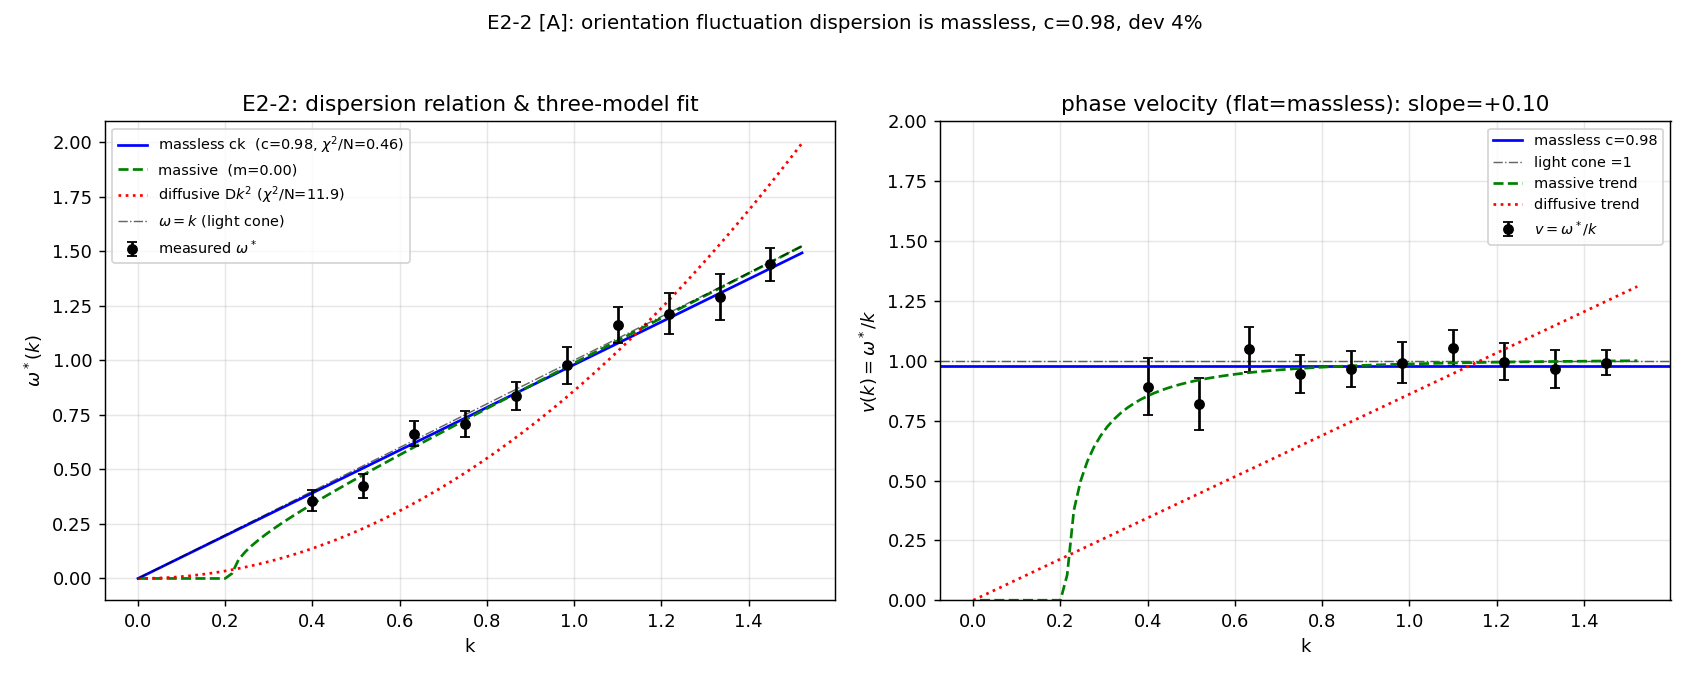
\includegraphics[width=\textwidth]{e2_dispersion.png}
\caption{Symbol of the causal wave operator: the on-shell zero crossing follows
$\omega=ck$ with a fitted light-cone speed (recovered without inserting $c$) and a
vanishing mass; the diffusive law $\omega=Dk^2$ is rejected. The dispersion is a
property of the operator built from the causal order.}\label{fig:disp}
\end{figure*}

\section{Polarisation: scalars, not a gauge vector}\label{sec:locking}

We now ask the structural question that the mode count alone cannot answer. The
ordering $O(3)\to O(2)$ leaves two gapless transverse modes, the number a photon
has; but a photon is a transverse \emph{vector} $A_i$ whose polarisation index is a
spatial index locked to the wavevector ($\vec k\!\cdot\!\vec\epsilon=0$), whereas
the two transverse modes of Eq.~\eqref{eq:action} carry an \emph{internal} index on
$S^2$ with, a priori, no relation to space. On symmetry grounds the global internal
$O(3)$ of Eq.~\eqref{eq:action} is decoupled from the spacetime Lorentz symmetry, so
the internal polarisation should be isotropic and independent of $\vec k$. We test
this directly.

\subsection{Estimator and null}
In the ordered state ($J=2.0$) we build the internal transverse frame
$(\vec e_1,\vec e_2)\perp\langle\vec n\rangle$ and the components $a_\alpha(i)=\vec
n_i\!\cdot\!\vec e_\alpha$ ($\alpha=1,2$). For $160$ wavevectors ($32$ directions
$\times5$ magnitudes) we form the $2\times2$ Hermitian polarisation tensor
\begin{equation}
\begin{split}
P_{\alpha\beta}(\vec k)&=\big\langle\, \mathrm{Re}_\alpha\mathrm{Re}_\beta
+\mathrm{Im}_\alpha\mathrm{Im}_\beta \,\big\rangle,\quad\text{with}\\
\mathrm{Re}_\alpha&=\sum_i a_\alpha(i)\cos(\vec k\!\cdot\!\vec x_i),\quad
\mathrm{Im}_\alpha=\sum_i a_\alpha(i)\sin(\vec k\!\cdot\!\vec x_i),
\end{split}
\label{eq:Ptensor}
\end{equation}
averaged over $16$ seeds $\times\,40$ samples, and its anisotropy
$r=(\lambda_1-\lambda_2)/(\lambda_1+\lambda_2)$ and principal-axis angle. A genuine
transverse vector locks the polarisation axis to $\hat k$; two decoupled internal
scalars do not. The clean, confound-free test is a permutation null: randomise the
$\hat k\leftrightarrow P$ pairing and ask whether the measured eigenvector--$\hat k$
correlation exceeds the null. (A position-shuffle baseline for the anisotropy
\emph{magnitude} is a confound: the ordered field has real-space coherence that the
shuffle destroys, inflating the apparent anisotropy excess without any locking; the
locking test is the correlation, not the magnitude.)

\subsection{Result: the photon is excluded}
The polarisation principal axis does \emph{not} track the spatial wavevector:
\begin{equation}
\text{eigvec--}\hat k\ \text{corr}=+0.10,\quad
\text{permutation } p=0.23\ (+0.7\sigma),
\label{eq:locking}
\end{equation}
i.e.\ consistent with random $\hat k\leftrightarrow$axis pairing
(Fig.~\ref{fig:locking}). (The anisotropy magnitude sits $9\sigma$ above the
position-shuffle baseline, but this is the real-space-coherence confound noted
above, not locking, as the permutation test makes explicit.)

\begin{figure*}[t]
\centering
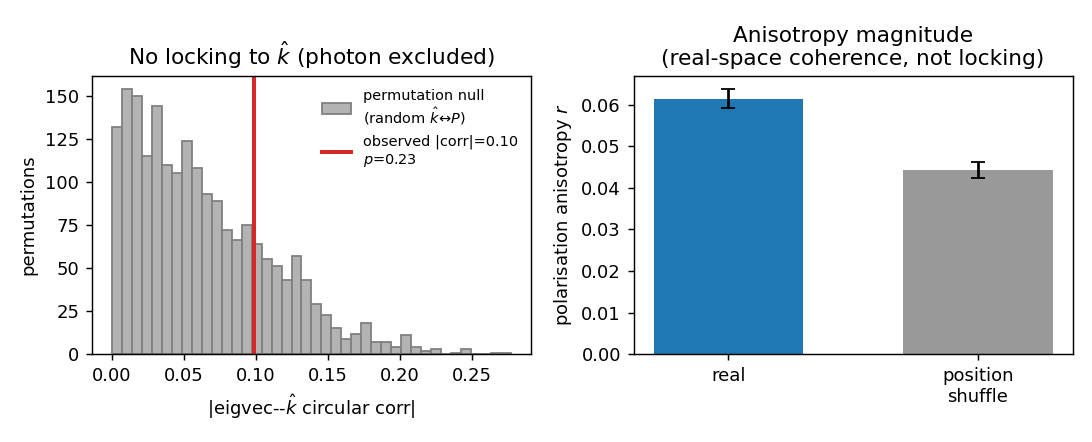
\includegraphics[width=\textwidth]{E4_1_locking.png}
\caption{The decisive polarisation test (E4-1). Left: the observed
eigenvector--$\hat k$ circular correlation (vertical line) sits inside the
permutation null obtained by randomising the $\hat k\leftrightarrow P$ pairing
($p=0.23$); the polarisation does \emph{not} lock to the wavevector---the signature
of a gauge vector is \emph{absent}. Right: the anisotropy magnitude exceeds the
position-shuffle baseline, but this reflects real-space field coherence (which the
shuffle destroys), not locking. The two transverse Goldstone modes are internal
scalars, not a photon.}\label{fig:locking}
\end{figure*} The two transverse Goldstone modes therefore carry an internal
polarisation unlocked from space: they are \emph{two decoupled internal scalars},
not a transverse gauge vector. The identification of these modes with the
photon---natural from the mode count, and which we had conjectured---is excluded by
this measurement. This is the expected outcome for a bare sigma model whose global
internal symmetry is decoupled from spacetime, and it is consistent with the model's
$SU(3)$ extension \cite{GellMann1962}, where the broken-generator Goldstones are the
pseudoscalar meson octet---i.e.\ this mechanism produces pion-like scalars, not a
photon.

\section{The scalar modes are degenerate and isotropic}\label{sec:degeneracy}

Having excluded the vector identification, we confirm the two modes form a clean
equivalent scalar pair. Measuring the per-mode transverse structure factor
$S_\alpha(\vec k)=\langle|\sum_i a_\alpha(i)e^{-i\vec k\cdot\vec x_i}|^2\rangle/N$
over $32$ directions and $6$ magnitudes ($16$ seeds $\times\,40$ samples), we find
the two modes degenerate to
$\langle|S_1-S_2|/(S_1+S_2)\rangle=0.037$ (required by the residual $O(2)$ symmetry
about $\langle\vec n\rangle$) and spatially isotropic, with a direction-to-direction
coefficient of variation of $0.042$ at fixed $|\vec k|$---emergent spatial isotropy
of the ordered vacuum. The transverse structure factor falls as
$S(k)\sim k^{-0.58}$ over the probed range; we report this as a diagnostic and do
not over-interpret it at the present size and six-point $k$-range (it is softer than
the mean-field flat value $0$ but does not yet reach the relativistic $1/k$; pinning
the stiffness exponent would require a dedicated larger-$N$, wider-$k$ study).
Figure~\ref{fig:isotropy} shows the two modes overlapping (degeneracy) and the
per-direction structure factors collapsing onto their mean (isotropy).

\begin{figure*}[t]
\centering
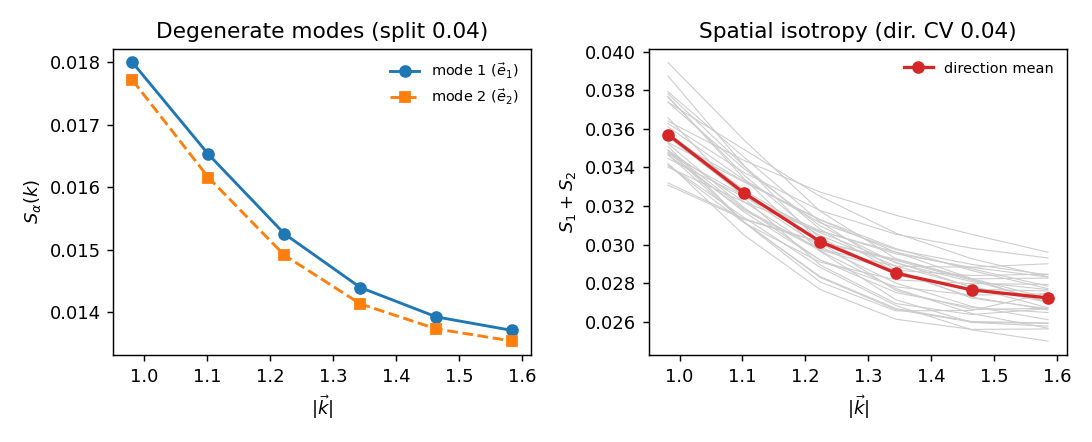
\includegraphics[width=\textwidth]{E4_2_isotropy.png}
\caption{Degeneracy and isotropy of the scalar modes (E4-2). Left: the
direction-averaged structure factors of the two transverse modes overlap (split
$3.7\%$)---they are degenerate, as the residual $O(2)$ symmetry requires. Right: the
transverse structure factor for each of $32$ spatial directions (grey) collapses
onto the direction mean (red), a $4.2\%$ coefficient of variation---emergent spatial
isotropy.}\label{fig:isotropy}
\end{figure*}

\section{Robustness checks}\label{sec:robust}

The results above were obtained at one sprinkling density and with the engine's
uniform link coupling. We verified by direct re-measurement that the two central
results---the genuine long-range order and the scalar, non-locking character of the
Goldstone modes---survive changing both, reusing the same engine without
modification (the criteria and outcomes are summarised in Table~\ref{tab:robust}).

\emph{Sprinkling density.} Repeating the finite-size-scaling order test at half and
twice the baseline density ($\rho=0.25$ and $\rho=1.0$) leaves the ordering intact:
the order parameter rises with $N$ at every density, stays $9$--$41\times$ above the
random floor, and $U_4=2/3$ to four digits throughout. The polarisation-locking test
likewise shows \emph{no} locking at any density (permutation $p=0.68,\,0.63,\,0.23$
at $\rho=0.25,\,0.5,\,1.0$): the photon exclusion is not an artefact of the chosen
density.

\emph{Coupling form.} The engine couples neighbours with a uniform weight, whereas
the action Eq.~\eqref{eq:action} carries a per-link proper-time weight
$\Delta\tau_{ij}$. Re-running the locking test with that proper-time-weighted
coupling---a genuinely different coupling form---again finds the polarisation
unlocked from $\hat k$ (permutation $p=0.76$). The scalar character, and hence the
retraction of the photon identification, is therefore not specific to the uniform
coupling.

\emph{Convergence with $N$.} Table~\ref{tab:fss} already exhibits the convergence
explicitly---$m(N)$ rising monotonically and $U_4=2/3$ at every size from $N=175$ to
$1462$; the density sweep extends the same behaviour to $N\approx2\times10^3$.

\begin{table}[t]
\caption{Robustness of the orientational order and of the photon exclusion. Each row
re-runs the engine of \S\ref{sec:order}--\ref{sec:locking} with one ingredient
changed. ``locking $p$'' is the permutation $p$-value of the eigenvector--$\hat k$
correlation (\S\ref{sec:locking}); $p>0.05$ means no locking, i.e.\ the modes remain
internal scalars. Ordering and the photon exclusion survive every variation.}
\label{tab:robust}
\begin{ruledtabular}
\begin{tabular}{lcccc}
Variation & $N$ range & $m$ range & $U_4$ & locking $p$ \\
\colrule
$\rho\times0.5$ ($\rho{=}0.25$)   & $92$--$416$   & $0.929$--$0.979$ & $0.667$ & $0.68$ \\
baseline ($\rho{=}0.5$)           & $185$--$835$  & $0.962$--$0.987$ & $0.667$ & $0.63$ \\
$\rho\times2$ ($\rho{=}1.0$)      & $372$--$1672$ & $0.978$--$0.992$ & $0.667$ & $0.23$ \\
$\Delta\tau$-weighted coupling    & $\sim\!830$   & ---              & ---     & $0.76$ \\
\end{tabular}
\end{ruledtabular}
\end{table}

The $O(3)$ sigma model on the causal Hasse graph is the minimal rotation-invariant
coupling; we have verified above that both the ordering transition and the scalar
character of the Goldstone modes are robust to halving and doubling the sprinkling
density and to replacing the uniform coupling with the proper-time-weighted one. The
result therefore characterises a class of causal-set ferromagnets, not a single
fine-tuned model.

\section{What is, and is not, established}\label{sec:claim}

\emph{Established by measurement.} (a) The orientation field on a causal set
spontaneously orders, and the order is genuine by finite-size scaling
(\S\ref{sec:order}). (b) A field governed by the causal wave operator disperses
relativistically, $\omega=ck$, with the light-cone speed recovered from a generator
that excludes it (\S\ref{sec:dispersion}). (c) The two transverse Goldstone modes
are degenerate, spatially isotropic, internal \emph{scalars}
(\S\ref{sec:locking}--\ref{sec:degeneracy}). Their polarisation does not lock to the
wavevector, so they are not a transverse gauge vector.

\emph{Not established---and a conjecture explicitly retracted.} These scalar modes
are \emph{not} a photon: there is no spatial vector index, no gauge redundancy, and
no locking to $\hat k$. We had previously conjectured the photon identification on
the strength of the mode count and the relativistic dispersion; the polarisation
measurement of \S\ref{sec:locking} excludes it, and we retract it. No electric
charge, gauge coupling, or conserved current is derived. The relativistic dispersion
is a property of the causal d'Alembertian, established via its symbol rather than by
a stable dynamical propagation of $\delta\vec n$. We have checked that the latter
does not exist as an explicit scheme: the symmetric smeared SBD operator is not a
positive operator---its spectrum is dominated by the wrong-sign (Lorentzian)
eigenvalues---so an explicit elliptic time-march grows without bound, while the
retarded recursion is non-normal. The symbol is therefore the correct stable
extraction of the on-shell $\omega=ck$; this is an intrinsic consequence of the
Lorentzian signature, not a removable numerical artifact. The structure-factor
exponent of \S\ref{sec:degeneracy} is a size-limited diagnostic, not a precision
result.

\section{Where an emergent photon must be sought}\label{sec:outlook}

The measurement points, by elimination, to where an emergent photon would have to
originate in this framework. A gauge vector requires a field carrying a spacetime
index with a gauge redundancy, which the orientation order parameter (an internal
$S^2$ vector) does not provide. The natural carrier is instead a \emph{connection}
on the causal links---a $U(1)$ link variable $\theta_{ij}$ in the spirit of lattice
gauge theory \cite{Wilson1974}---whose excitation carries a genuine spacetime index
and a gauge redundancy, and whose Wilson loops define the field strength. Testing
whether such a link-connection sector on the causal set supports a massless
transverse vector with a Coulomb phase is a well-posed, separate programme, carried
out in the companion paper~\cite{PhotonArcCQG}, which maps this sector systematically
(causal diamonds are found to be $100\%$ electric, the Anderson--Higgs route is
frustrated by the operator's non-locality, and a magnetic sector emerges only under
sub-Planckian curvature). Equivalently, forcing the orientation field itself to
yield a vector would require an added internal--spatial (spin--orbit) locking term;
that is an external ingredient, not one the bare substrate supplies.

\section{Conclusions}\label{sec:conclusions}

Equipping the causal set with a single internal orientation, and analysing it under
a guard that forbids inserting relativity, we have established by measurement that
the orientation vacuum spontaneously orders---genuinely, by finite-size
scaling---and that a field governed by the causal wave operator disperses
relativistically, with the light-cone speed an output rather than an input. We then
tested the tensorial character of the two transverse Goldstone modes and found,
through a polarisation tensor and a confound-free permutation null, that they do not
lock to the spatial wavevector: they are two degenerate, spatially isotropic,
internal scalar Goldstone bosons, not a transverse gauge vector. We therefore
exclude---and retract---the identification of these modes with the photon, and we
locate the emergent-photon question in the gauge-connection (link-variable) sector
instead, where the companion paper~\cite{PhotonArcCQG} pursues it. The positive content stands on its own: a discrete causal substrate,
reused without modification from causal set theory, supports a vacuum with genuine
spontaneous internal order whose Goldstone excitations are relativistic scalars,
consistent with the pseudoscalar sector of the model's non-Abelian extension.

\begin{acknowledgments}
This work uses only the author's own simulations; the anti-circularity guard, the
validation gates, and the pre-registered decision criteria of the E4 campaign are
part of the build.
\end{acknowledgments}

\bibliographystyle{apsrev4-2}
\bibliography{TEIC_CONSOLIDATED}

\end{document}
